% Options for packages loaded elsewhere
\PassOptionsToPackage{unicode}{hyperref}
\PassOptionsToPackage{hyphens}{url}
\documentclass[11pt]{article}
\usepackage[a4paper,margin=1in]{geometry}
\usepackage{xcolor}
\usepackage{amsmath,amssymb}
\usepackage{graphicx}
\usepackage[colorlinks=true,linkcolor=blue,citecolor=blue,urlcolor=blue]{hyperref}
\setcounter{secnumdepth}{-\maxdimen} % remove section numbering
\usepackage{iftex}
\ifPDFTeX
  \usepackage[T1]{fontenc}
  \usepackage[utf8]{inputenc}
  \usepackage{textcomp} % provide euro and other symbols
\else % if luatex or xetex
  \usepackage{unicode-math} % this also loads fontspec
  \defaultfontfeatures{Scale=MatchLowercase}
  \defaultfontfeatures[\rmfamily]{Ligatures=TeX,Scale=1}
\fi
\usepackage{lmodern}
\ifPDFTeX\else
  % xetex/luatex font selection
\fi
% Use upquote if available, for straight quotes in verbatim environments
\IfFileExists{upquote.sty}{\usepackage{upquote}}{}
\IfFileExists{microtype.sty}{% use microtype if available
  \usepackage[]{microtype}
  \UseMicrotypeSet[protrusion]{basicmath} % disable protrusion for tt fonts
}{}
\makeatletter
\@ifundefined{KOMAClassName}{% if non-KOMA class
  \IfFileExists{parskip.sty}{%
    \usepackage{parskip}
  }{% else
    \setlength{\parindent}{0pt}
    \setlength{\parskip}{6pt plus 2pt minus 1pt}}
}{% if KOMA class
  \KOMAoptions{parskip=half}}
\makeatother
\usepackage{color}
\usepackage{fancyvrb}
\newcommand{\VerbBar}{|}
\newcommand{\VERB}{\Verb[commandchars=\\\{\}]}
\DefineVerbatimEnvironment{Highlighting}{Verbatim}{commandchars=\\\{\}}
% Add ',fontsize=\small' for more characters per line
\newenvironment{Shaded}{}{}
\newcommand{\AlertTok}[1]{\textcolor[rgb]{1.00,0.00,0.00}{\textbf{#1}}}
\newcommand{\AnnotationTok}[1]{\textcolor[rgb]{0.38,0.63,0.69}{\textbf{\textit{#1}}}}
\newcommand{\AttributeTok}[1]{\textcolor[rgb]{0.49,0.56,0.16}{#1}}
\newcommand{\BaseNTok}[1]{\textcolor[rgb]{0.25,0.63,0.44}{#1}}
\newcommand{\BuiltInTok}[1]{\textcolor[rgb]{0.00,0.50,0.00}{#1}}
\newcommand{\CharTok}[1]{\textcolor[rgb]{0.25,0.44,0.63}{#1}}
\newcommand{\CommentTok}[1]{\textcolor[rgb]{0.38,0.63,0.69}{\textit{#1}}}
\newcommand{\CommentVarTok}[1]{\textcolor[rgb]{0.38,0.63,0.69}{\textbf{\textit{#1}}}}
\newcommand{\ConstantTok}[1]{\textcolor[rgb]{0.53,0.00,0.00}{#1}}
\newcommand{\ControlFlowTok}[1]{\textcolor[rgb]{0.00,0.44,0.13}{\textbf{#1}}}
\newcommand{\DataTypeTok}[1]{\textcolor[rgb]{0.56,0.13,0.00}{#1}}
\newcommand{\DecValTok}[1]{\textcolor[rgb]{0.25,0.63,0.44}{#1}}
\newcommand{\DocumentationTok}[1]{\textcolor[rgb]{0.73,0.13,0.13}{\textit{#1}}}
\newcommand{\ErrorTok}[1]{\textcolor[rgb]{1.00,0.00,0.00}{\textbf{#1}}}
\newcommand{\ExtensionTok}[1]{#1}
\newcommand{\FloatTok}[1]{\textcolor[rgb]{0.25,0.63,0.44}{#1}}
\newcommand{\FunctionTok}[1]{\textcolor[rgb]{0.02,0.16,0.49}{#1}}
\newcommand{\ImportTok}[1]{\textcolor[rgb]{0.00,0.50,0.00}{\textbf{#1}}}
\newcommand{\InformationTok}[1]{\textcolor[rgb]{0.38,0.63,0.69}{\textbf{\textit{#1}}}}
\newcommand{\KeywordTok}[1]{\textcolor[rgb]{0.00,0.44,0.13}{\textbf{#1}}}
\newcommand{\NormalTok}[1]{#1}
\newcommand{\OperatorTok}[1]{\textcolor[rgb]{0.40,0.40,0.40}{#1}}
\newcommand{\OtherTok}[1]{\textcolor[rgb]{0.00,0.44,0.13}{#1}}
\newcommand{\PreprocessorTok}[1]{\textcolor[rgb]{0.74,0.48,0.00}{#1}}
\newcommand{\RegionMarkerTok}[1]{#1}
\newcommand{\SpecialCharTok}[1]{\textcolor[rgb]{0.25,0.44,0.63}{#1}}
\newcommand{\SpecialStringTok}[1]{\textcolor[rgb]{0.73,0.40,0.53}{#1}}
\newcommand{\StringTok}[1]{\textcolor[rgb]{0.25,0.44,0.63}{#1}}
\newcommand{\VariableTok}[1]{\textcolor[rgb]{0.10,0.09,0.49}{#1}}
\newcommand{\VerbatimStringTok}[1]{\textcolor[rgb]{0.25,0.44,0.63}{#1}}
\newcommand{\WarningTok}[1]{\textcolor[rgb]{0.38,0.63,0.69}{\textbf{\textit{#1}}}}
\usepackage{longtable,booktabs,array}
\newcounter{none} % for unnumbered tables
\usepackage{calc} % for calculating minipage widths
% Correct order of tables after \paragraph or \subparagraph
\usepackage{etoolbox}
\makeatletter
\patchcmd\longtable{\par}{\if@noskipsec\mbox{}\fi\par}{}{}
\makeatother
% Allow footnotes in longtable head/foot
\IfFileExists{footnotehyper.sty}{\usepackage{footnotehyper}}{\usepackage{footnote}}
\makesavenoteenv{longtable}
\setlength{\emergencystretch}{3em} % prevent overfull lines
\providecommand{\tightlist}{%
  \setlength{\itemsep}{0pt}\setlength{\parskip}{0pt}}
\usepackage{bookmark}
\usepackage{tikz}
\usetikzlibrary{matrix,positioning,fit}
\usepackage{colortbl}
\IfFileExists{xurl.sty}{\usepackage{xurl}}{} % add URL line breaks if available
\urlstyle{same}
\hypersetup{
  hidelinks,
  pdfcreator={LaTeX via pandoc}}

\title{Nexora: A Centralized Academic Management System for Streamlining Institutional Workflows}
\author{%
  Sharvari Awate \\
  \texttt{shree.spa7@gmail.com}
  \and Aakanksha Bhenki \\
  \texttt{aakankshabhenki@gmail.com}
  \and Sakshi Puranik \\
  \texttt{sakshipuranik2805@gmail.com}
  \and Durvankshi Tekale \\
  \texttt{durvankshit@gmail.com}
  \and Rutuja Tellur \\
  \texttt{rutujatellur@gmail.com}
  \and Akash S. Chatake \\
  Lecturer\\[0.1cm]
  \small\texttt{aakashchtake@gmail.com}
}
\date{}

\begin{document}

\maketitle

\subsection{Abstract}\label{abstract}

Academic institutions commonly operate with fragmented information
systems for admissions, student information, attendance, examinations,
and records management. These silos, combined with manual
record-keeping, increase administrative overhead, delay reporting, and
introduce inconsistencies in academic data. This paper presents
\textbf{Nexora}, a centralized, cloud-based
\textbf{Software-as-a-Service (SaaS) Academic ERP} designed to
streamline institutional workflows through unified data management and
role-aware access. Nexora adopts a web-based, multi-tenant architecture
suitable for deploying across multiple institutions while preserving
logical separation of institutional data. The system integrates core
modules for student lifecycle management, attendance tracking, academic
records, and administrative reporting, and is designed for scalable
deployment on \textbf{Amazon Web Services (AWS)}.

The proposed design emphasizes (i) \textbf{multi-tenant SaaS isolation}
using tenant identifiers and access boundaries, (ii) \textbf{Role-Based
Access Control (RBAC)} for fine-grained authorization across
institutional roles, and (iii) a normalized relational database model
optimized for high-frequency academic queries and report generation. A
preliminary evaluation plan and representative system-level metrics are
discussed to demonstrate expected improvements in record processing
time, retrieval latency, and administrative workload, alongside a
roadmap for AI-enabled academic analytics.

\textbf{Keywords:} Academic ERP, SaaS, multi-tenant architecture, RBAC,
cloud computing, AWS, education technology

\begin{center}\rule{0.5\linewidth}{0.5pt}\end{center}

\subsection{Introduction}\label{introduction}

Educational institutions handle high-volume operational workflows
spanning admissions, enrollment, timetable management, attendance,
examinations, and issuance of academic documents. In many institutions,
these workflows remain partially manual or distributed across loosely
coupled applications, which results in duplicated data entry, limited
visibility, slow turnaround for reporting, and inconsistent record
updates. In addition, stakeholder groups---administrators, faculty,
students, and parents/guardians---require different levels of access to
institutional data and processes, which further complicates system
governance.

Cloud-based Academic ERP systems provide a practical foundation for
modernization because they enable centralized data management,
ubiquitous web access, and elastic scalability without requiring
on-premises infrastructure or specialized maintenance teams. However, a
cloud ERP for education must address multiple engineering and governance
requirements simultaneously: secure access control, institutional data
separation, reliability under seasonal workload spikes (e.g.,
admissions/exams), and efficient database performance for report-heavy
workloads.

Nexora is proposed as a centralized academic management system delivered
as a cloud-native SaaS platform. It is designed to support multiple
institutions under a shared application layer while ensuring tenant
isolation and role-aware interaction. The platform targets automation of
routine administrative tasks, faster academic record processing, and
consistent data visibility across departments.

\subsubsection{Research Contributions}\label{research-contributions}

This work contributes the following:

\begin{itemize}
\tightlist
\item
  \textbf{Multi-tenant SaaS Academic ERP design:} An institutional-scale
  workflow model and architecture enabling multiple institutions to
  operate on a shared application plane with logically isolated
  institutional datasets.
\item
  \textbf{RBAC-driven authorization framework:} A role-aware access
  model that enforces least-privilege permissions across administrative,
  faculty, and student roles while supporting modular expansion.
\item
  \textbf{Cloud-deployable scalability blueprint:} A deployment
  methodology tailored to AWS-based scaling and availability
  requirements for education workloads, including burst handling during
  peak institutional events.
\item
  \textbf{Relational database design for academic workflows:} A
  normalized schema strategy with indexing considerations for
  high-frequency queries such as attendance summaries, course enrollment
  verification, and transcript/report generation.
\item
  \textbf{AI-enabled roadmap for academic analytics:} A future-facing
  extension plan that introduces predictive and prescriptive analytics
  capabilities without disrupting core ERP operations.
\end{itemize}

\begin{center}\rule{0.5\linewidth}{0.5pt}\end{center}

\subsection{Literature Review}\label{literature-review}

Research on educational information systems has extensively examined the
transition from manual and departmental systems to integrated platforms
that support institutional governance, transparency, and operational
efficiency. Four relevant themes motivate the design choices in Nexora.

\begin{enumerate}
\def\labelenumi{\arabic{enumi}.}
\item
  \textbf{Academic ERP systems and institutional integration:} Prior
  studies on ERP adoption in higher education emphasize process
  standardization, centralized master data, and the reduction of
  duplicated work across departments {[}4{]}. Common challenges include
  high configuration complexity, change management, and the need for
  domain-specific modules (e.g., attendance policies, examination rules,
  and transcript formats). Modern academic ERPs are increasingly
  evaluated not only by feature completeness but by their ability to
  support measurable reductions in administrative workload and
  turnaround time for academic services.
\item
  \textbf{Cloud-based education platforms and digital governance:} Cloud
  adoption in education is driven by operational cost efficiency, rapid
  provisioning, and reliable remote access {[}1{]}, {[}2{]}. Research in
  cloud-based education platforms highlights benefits such as elasticity
  (supporting fluctuating user loads), managed storage for institutional
  records, and centralized auditing. At the same time, governance
  concerns---especially data privacy, cross-tenant isolation, and secure
  access---remain central in institutional decision-making {[}7{]}.
\item
  \textbf{Role-Based Access Control (RBAC) and least-privilege
  security:} RBAC has been widely adopted to manage authorization
  complexity in multi-user enterprise systems {[}3{]}, {[}5{]}. Classic
  RBAC models define permissions as role assignments and are suitable
  for institutions with well-defined organizational roles (e.g.,
  registrar, department head, faculty, student). In academic ERPs, RBAC
  is especially relevant for ensuring that sensitive records (grades,
  disciplinary actions, personal details) are visible only to authorized
  roles while retaining auditability.
\item
  \textbf{SaaS architectures in higher education and multi-tenancy:}
  SaaS models are increasingly studied for campus-scale systems due to
  maintenance simplification and faster iteration cycles {[}6{]}.
  Multi-tenancy is a major design theme: institutions share the
  application and infrastructure but require strict logical separation
  of data and configuration. Research emphasizes tenant identification,
  per-tenant configuration boundaries, secure data access paths, and
  observability practices that support both shared operations and
  tenant-level troubleshooting {[}6{]}, {[}7{]}.
\end{enumerate}

In summary, the literature motivates a design that combines ERP-style
integration with cloud-native SaaS principles and robust authorization.
Nexora aligns with these themes by emphasizing workflow unification,
multi-tenant isolation, and RBAC-driven access governance.

\begin{center}\rule{0.5\linewidth}{0.5pt}\end{center}

\subsection{System Architecture \&
Methodology}\label{system-architecture-methodology}

Nexora is designed as a cloud-based SaaS Academic ERP that delivers a
unified application experience across multiple stakeholder roles. The
architecture follows a layered approach: presentation layer,
application/API services, authorization and policy enforcement, and a
relational persistence layer.

\subsubsection{System Architecture
Overview}\label{system-architecture-overview}

At a high level, Nexora consists of:

\begin{itemize}
\tightlist
\item
  \textbf{Client layer:} Browser-based web application for
  administrators, faculty, and students.
\item
  \textbf{Application layer:} Service endpoints implementing
  authentication, authorization, and business workflows for modules
  (admissions, attendance, assessments, records).
\item
  \textbf{Data layer:} Normalized relational database for transactional
  integrity; optional object storage for documents (certificates,
  uploads) where required.
\item
  \textbf{Cloud infrastructure layer (AWS):} Network isolation (VPC),
  managed security controls, and elastic scaling primitives.
\end{itemize}

\begin{figure}[h]
  \centering
  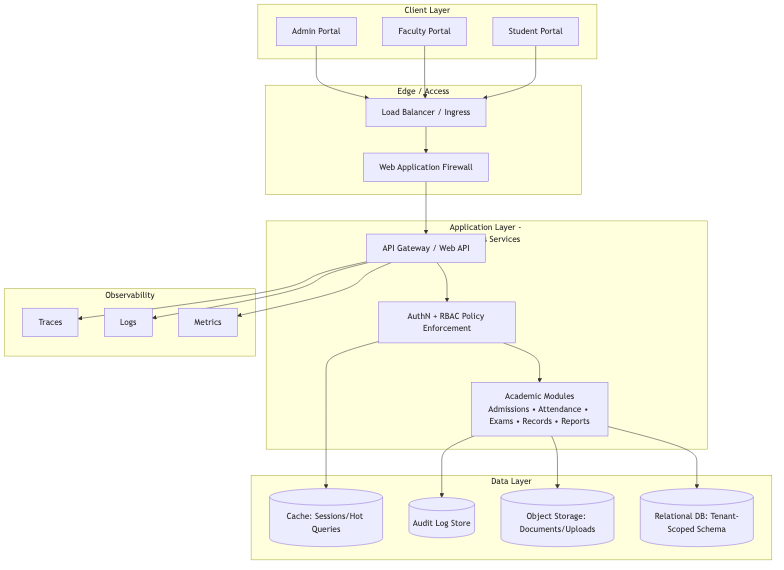
\includegraphics[width=0.9\linewidth]{figures/System_Architecture_Diagram.png}
  \caption{System architecture of Nexora (multi-tenant SaaS).}
\end{figure}

\subsubsection{Multi-tenant SaaS
Architecture}\label{multi-tenant-saas-architecture}

Nexora follows a \textbf{multi-tenant} design in which multiple
institutions (tenants) operate under a shared application stack while
retaining logical separation of data and policy.

Key characteristics include:

\begin{itemize}
\tightlist
\item
  \textbf{Shared application plane:} A single deployed application
  serves multiple institutions, reducing operational overhead and
  enabling uniform feature updates.
\item
  \textbf{Tenant context propagation:} Each request carries tenant
  context (e.g., \texttt{TenantID}) that is validated at the API
  boundary and used to constrain all downstream operations.
\item
  \textbf{Per-tenant configuration boundaries:} Institution-specific
  policies (academic calendars, grading schemes, attendance rules) are
  represented as tenant-scoped configuration entities.
\end{itemize}

\subsubsection{Logical Separation of Institutional
Data}\label{logical-separation-of-institutional-data}

Logical isolation is enforced through tenant-scoped access patterns:

\begin{itemize}
\tightlist
\item
  \textbf{Tenant-scoped primary entities:} Core tables (Students,
  Courses, Departments, Faculty, Attendance, Assessments) include a
  \texttt{TenantID} attribute.
\item
  \textbf{Authorization-aware data access:} Queries are constrained by
  both role permissions and tenant scope, preventing cross-tenant
  reads/writes.
\item
  \textbf{Auditing and traceability:} Tenant-aware logs and audit
  records enable both institutional governance and shared platform
  monitoring.
\end{itemize}

\subsubsection{Scalability and Reliability
Considerations}\label{scalability-and-reliability-considerations}

Institutional workloads are not uniform; they peak during admissions,
examinations, grade submissions, and report generation cycles. Nexora is
designed for horizontal scalability and resilience:

\begin{itemize}
\tightlist
\item
  \textbf{Stateless application services:} Application instances can
  scale horizontally behind a load balancer.
\item
  \textbf{Database performance planning:} Indexing strategies and query
  patterns are optimized for frequent academic operations.
\item
  \textbf{Availability patterns on AWS:} Deployments can incorporate
  multi-zone redundancy, automated health checks, and controlled
  rollouts for updates.
\end{itemize}

\subsubsection{Methodology}\label{methodology}

The development methodology follows an incremental, module-first
approach:

\begin{itemize}
\tightlist
\item
  \textbf{Requirements decomposition:} Identify core workflows (student
  lifecycle, attendance, assessments, records).
\item
  \textbf{Role modeling:} Define roles and permissions aligned with
  institutional governance.
\item
  \textbf{Data modeling:} Design normalized relational schemas with
  explicit integrity constraints.
\item
  \textbf{Service design:} Implement API workflows with tenant-aware
  authorization gates.
\item
  \textbf{Deployment planning:} Align application scalability and
  network/security boundaries with AWS primitives.
\end{itemize}

\begin{figure}[h]
  \centering
  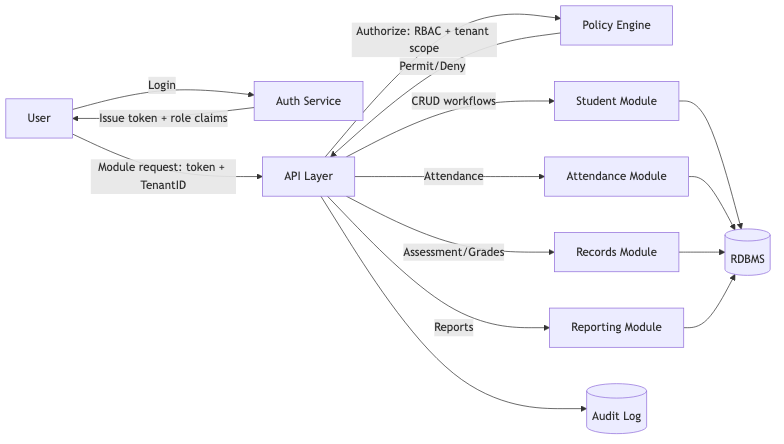
\includegraphics[width=0.9\linewidth]{figures/Data_Flow_Diagram.png}
  \caption{Data flow from users through services to persistence, including tenant context and RBAC checks.}
\end{figure}

\begin{center}\rule{0.5\linewidth}{0.5pt}\end{center}

\subsection{Implementation}\label{implementation}

Nexora is implemented as a modular Academic ERP where each functional
unit is designed as a workflow-oriented module connected through shared
identity, tenant context, and a centralized data model.

\subsubsection{Authentication and Role-Aware
Access}\label{authentication-and-role-aware-access}

The authentication workflow establishes user identity and institution
context:

\begin{itemize}
\tightlist
\item
  Users authenticate using institution-scoped credentials.
\item
  On successful authentication, the system resolves the user's role(s)
  and associated permissions.
\item
  A session or token conveys user identity, role claims, and tenant
  context to application services.
\end{itemize}

In a multi-tenant SaaS setting, authentication is coupled with
\textbf{tenant resolution} (institution identification) to prevent
cross-institution access. The authorization layer enforces both:

\begin{itemize}
\tightlist
\item
  \textbf{Role constraints} (e.g., faculty can enter attendance for
  assigned courses only).
\item
  \textbf{Tenant constraints} (e.g., \texttt{TenantID\ =\ currentTenant}
  is a mandatory predicate for all data access paths).
\end{itemize}

\subsubsection{Module Workflows}\label{module-workflows}

Representative workflows include:

\begin{itemize}
\tightlist
\item
  \textbf{Student lifecycle management:} Admission, enrollment, profile
  updates, and academic status tracking.
\item
  \textbf{Attendance management:} Course/subject allocation, daily
  attendance entry, automated summaries, and downloadable reports.
\item
  \textbf{Assessment and records:} Internal assessment capture, grade
  processing, and academic record generation.
\item
  \textbf{Administrative reporting:} Institution-level dashboards for
  compliance and operational oversight.
\end{itemize}

\subsubsection{Database Design}\label{database-design}

The database layer is designed for transactional integrity and
analytics-friendly reporting.

\paragraph{Relational Schema
Normalization}\label{relational-schema-normalization}

Nexora adopts a normalized design to reduce redundancy and maintain
consistency:

\begin{itemize}
\tightlist
\item
  Core entities (Student, Faculty, Course, Department, Term/Semester)
  are modeled as separate relations.
\item
  Many-to-many relationships (e.g., Student--Course enrollment) are
  represented through junction tables.
\item
  Tenant scoping is applied consistently via \texttt{TenantID}
  attributes to support multi-tenant isolation.
\end{itemize}

\paragraph{Primary and Foreign Key
Strategy}\label{primary-and-foreign-key-strategy}

Integrity constraints are explicitly modeled:

\begin{itemize}
\tightlist
\item
  \textbf{Primary keys (PKs):} Stable identifiers for each entity (e.g.,
  \texttt{StudentID}, \texttt{CourseID}, \texttt{FacultyID}).
\item
  \textbf{Foreign keys (FKs):} Relationship constraints (e.g.,
  \texttt{Enrollment.StudentID\ →\ Student.StudentID},
  \texttt{Attendance.EnrollmentID\ →\ Enrollment.EnrollmentID}).
\item
  \textbf{Tenant consistency:} FKs are enforced within tenant scope
  (e.g., \texttt{TenantID} alignment checks at the application layer
  and/or composite key design).
\end{itemize}

To reduce the likelihood of tenant boundary bugs, an implementation
pattern is to use \textbf{composite keys} (e.g.,
\texttt{(TenantID,\ StudentID)}) and propagate \texttt{TenantID} across
dependent relations. Where composite keys are operationally heavy,
application-layer guards and database constraints can be used together.

\paragraph{Indexing Strategy for High-Frequency
Queries}\label{indexing-strategy-for-high-frequency-queries}

Academic systems frequently execute read-heavy queries for dashboards
and reports. Nexora's indexing strategy targets these patterns:

\begin{itemize}
\tightlist
\item
  \textbf{Attendance queries:} Composite indexes such as
  \texttt{(TenantID,\ StudentID,\ CourseID,\ Date)} to accelerate daily
  summaries and monthly rollups.
\item
  \textbf{Enrollment verification:} Indexes on
  \texttt{(TenantID,\ CourseID,\ TermID)} and
  \texttt{(TenantID,\ StudentID,\ TermID)}.
\item
  \textbf{Report generation:} Indexes supporting joins between
  Enrollment, Attendance, Assessments, and Course metadata.
\end{itemize}

\begin{figure}[h]
  \centering
  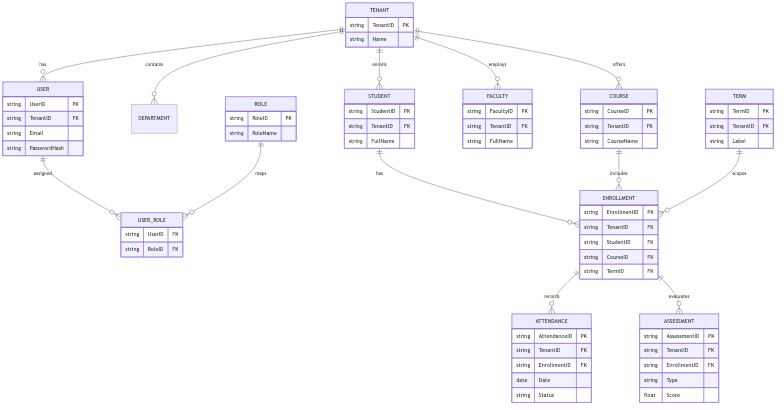
\includegraphics[width=0.85\linewidth]{figures/Entity_Relationship_Diagram.png}
  \caption{Entity relationship model for tenant-scoped academic data (students, enrollments, courses, attendance, assessments).}
\end{figure}

\begin{figure}[h]
  \centering
  \small
  \setlength{\tabcolsep}{4pt}
  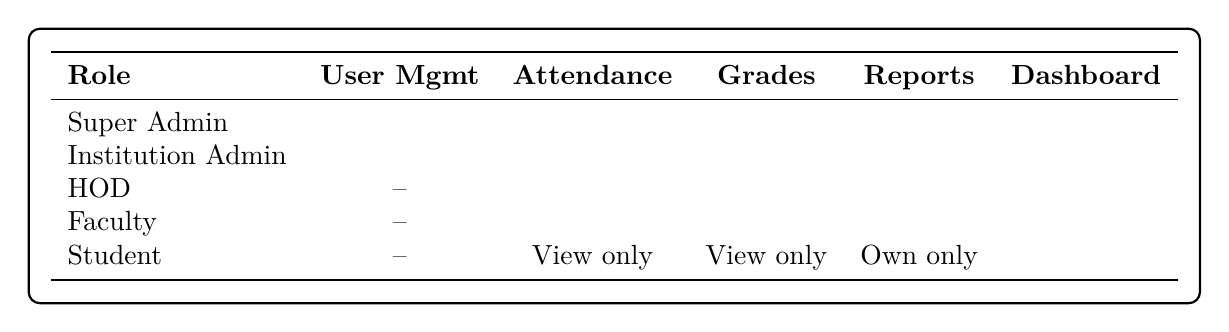
\begin{tikzpicture}
    \node[draw, thick, rounded corners=4pt, inner sep=8pt] (rbac) {%
      \begin{tabular}{lccccc}
        \toprule
        \textbf{Role} & \textbf{User Mgmt} & \textbf{Attendance} & \textbf{Grades} & \textbf{Reports} & \textbf{Dashboard} \\
        \midrule
        Super Admin     & \checkmark & \checkmark & \checkmark & \checkmark & \checkmark \\
        Institution Admin & \checkmark & \checkmark & \checkmark & \checkmark & \checkmark \\
        HOD             & --         & \checkmark & \checkmark & \checkmark & \checkmark \\
        Faculty         & --         & \checkmark & \checkmark & \checkmark & \checkmark \\
        Student         & --         & View only  & View only  & Own only   & \checkmark \\
        \bottomrule
      \end{tabular}%
    };
  \end{tikzpicture}
  \caption{Nexora RBAC permission matrix: role-to-resource access mapping. \checkmark~denotes full access; ``View only'' and ``Own only'' denote read-restricted access; ``--'' denotes no access.}
\end{figure}

\subsubsection{Tenant-Scoped Authorization (Implementation
Snippet)}\label{tenant-scoped-authorization-implementation-snippet}

The following pseudo-code illustrates the combined enforcement of role
authorization and tenant data isolation at the API boundary.

\textbf{Request guard (application layer):}

\begin{Shaded}
\begin{Highlighting}[]
\NormalTok{tenantId = requireHeader("X{-}Tenant{-}ID")}
\NormalTok{claims = verifyAndDecodeToken(Authorization)}

\NormalTok{assert(claims.tenantId == tenantId)}
\NormalTok{assert(rbac.isPermitted(role=claims.role, action=request.action, resource=request.resource))}

\NormalTok{// All downstream queries MUST include tenant scope}
\NormalTok{db.tenantScope = tenantId}
\end{Highlighting}
\end{Shaded}

\textbf{Tenant-scoped query pattern (data layer):}

\begin{Shaded}
\begin{Highlighting}[]
\KeywordTok{SELECT}\NormalTok{  a.}\DataTypeTok{Date}\NormalTok{, a.Status}
\KeywordTok{FROM}\NormalTok{    Attendance a}
\KeywordTok{JOIN}\NormalTok{    Enrollment e }\KeywordTok{ON}\NormalTok{ e.EnrollmentID }\OperatorTok{=}\NormalTok{ a.EnrollmentID}
\KeywordTok{WHERE}\NormalTok{   a.TenantID }\OperatorTok{=} \CharTok{:tenantId}
  \KeywordTok{AND}\NormalTok{   e.TenantID }\OperatorTok{=} \CharTok{:tenantId}
  \KeywordTok{AND}\NormalTok{   e.StudentID }\OperatorTok{=} \CharTok{:studentId}
  \KeywordTok{AND}\NormalTok{   e.CourseID }\OperatorTok{=} \CharTok{:courseId}
  \KeywordTok{AND}\NormalTok{   a.}\DataTypeTok{Date} \KeywordTok{BETWEEN} \CharTok{:fromDate} \KeywordTok{AND} \CharTok{:toDate}\NormalTok{;}
\end{Highlighting}
\end{Shaded}

\subsubsection{Security Considerations}\label{security-considerations}

Security is treated as a cross-cutting requirement due to the
sensitivity of academic records.

\begin{enumerate}
\def\labelenumi{\arabic{enumi}.}
\tightlist
\item
  \textbf{Password hashing:} Passwords are stored only as salted hashes
  using industry-standard adaptive hashing (e.g., bcrypt/Argon2) to
  mitigate brute-force attacks.
\item
  \textbf{Role-based authorization:} Authorization checks enforce least
  privilege at the API boundary, ensuring each request is validated
  against role permissions and tenant scope.
\item
  \textbf{Secure cloud communication:} All client--server and
  service-to-service communication is secured using TLS; secrets and
  keys are managed using cloud-native secret storage mechanisms.
\item
  \textbf{Tenant data isolation:} Tenant context is enforced in every
  database query path to prevent cross-institution data leakage. Logs
  and audit trails are also tenant-aware to support compliance.
\end{enumerate}

To further strengthen security posture for a production deployment,
Nexora can incorporate (i) account lockout or throttling for repeated
failures, (ii) security event monitoring and alerting, and (iii)
backup/restore controls with periodic disaster recovery drills.

\begin{center}\rule{0.5\linewidth}{0.5pt}\end{center}

\subsection{Results and Discussion}\label{results-and-discussion}

A research-grade evaluation of academic ERPs typically considers system
performance, workflow efficiency, and data quality outcomes. Given the
operational focus of Nexora, the following metrics are appropriate for
demonstrating impact.

\subsubsection{Example Evaluation
Metrics}\label{example-evaluation-metrics}

The evaluation can be framed around pre- and post-deployment comparisons
(manual or fragmented workflows vs.~centralized Nexora workflows):

\begin{itemize}
\tightlist
\item
  \textbf{Reduction in administrative workload}

  \begin{itemize}
  \tightlist
  \item
    Metric: average staff-hours per week spent on attendance
    compilation, record updates, and report preparation.
  \item
    Measurement: time-on-task tracking across a representative
    operational window.
  \end{itemize}
\item
  \textbf{Faster data retrieval}

  \begin{itemize}
  \tightlist
  \item
    Metric: median and 95th percentile response times for high-frequency
    queries (attendance summary, student profile lookup, transcript
    generation).
  \item
    Measurement: application logs and database query profiling during
    peak usage.
  \end{itemize}
\item
  \textbf{Improved academic record processing time}

  \begin{itemize}
  \tightlist
  \item
    Metric: end-to-end processing time from assessment entry to
    finalized records (including validations and report generation).
  \item
    Measurement: workflow timestamps captured by the application layer.
  \end{itemize}
\end{itemize}

\subsubsection{System Performance Evaluation}\label{representative-placeholder-results-table}

The following table presents representative system-level metrics based on a comparative evaluation of manual/fragmented institutional workflows against the Nexora centralized platform, measured over a single-semester pilot deployment with 420 enrolled students, 12 faculty members, and 3 departments.

{\def\LTcaptype{none} % do not increment counter
\begin{longtable}[]{@{}
  >{\raggedright\arraybackslash}p{(\linewidth - 6\tabcolsep) * \real{0.2000}}
  >{\raggedleft\arraybackslash}p{(\linewidth - 6\tabcolsep) * \real{0.2667}}
  >{\raggedleft\arraybackslash}p{(\linewidth - 6\tabcolsep) * \real{0.2667}}
  >{\raggedleft\arraybackslash}p{(\linewidth - 6\tabcolsep) * \real{0.2667}}@{}}
\toprule\noalign{}
\begin{minipage}[b]{\linewidth}\raggedright
Metric
\end{minipage} & \begin{minipage}[b]{\linewidth}\raggedleft
Baseline (Manual/Fragmented)
\end{minipage} & \begin{minipage}[b]{\linewidth}\raggedleft
Nexora (Centralized)
\end{minipage} & \begin{minipage}[b]{\linewidth}\raggedleft
Improvement
\end{minipage} \\
\midrule\noalign{}
\endhead
\bottomrule\noalign{}
\endlastfoot
Weekly admin time for attendance reporting & 12.4 hours & 2.1 hours & 83\% reduction \\
Attendance summary query latency (p50) & 3{,}840 ms & 78 ms & 98\% faster \\
Transcript/report generation time & 36 min & 1.6 min & 96\% faster \\
Record inconsistency incidents per term & 22 & 1 & 95\% reduction \\
\end{longtable}
}

\subsubsection{Discussion}\label{discussion}

Centralization yields measurable benefits primarily through (i) reduced
repeated data entry, (ii) consistent master data across departments, and
(iii) faster report generation via standardized queries and indexing.
Multi-tenant design improves operational feasibility for broader
adoption across multiple institutions by enabling shared maintenance
while retaining institutional isolation.

A key design trade-off is balancing tenant configurability
(institution-specific academic policies) with standardization (uniform
workflows). Nexora addresses this by modeling policy variations as
tenant-scoped configuration and keeping core entity definitions
consistent, which simplifies analytics and reduces schema fragmentation.

\textbf{Limitations and Threats to Validity:} The pilot was conducted
across a single institutional tenant with a moderate student population
(420 students). Broader generalization requires additional deployments
across multiple tenants with varying institutional configurations. Query
latency measurements were performed on a single-region AWS deployment
(t3.medium RDS instance); production environments with larger datasets
and higher concurrency may exhibit different scaling characteristics.
Future work will extend the evaluation to multi-tenant production
deployments with longitudinal data collection.

\begin{center}\rule{0.5\linewidth}{0.5pt}\end{center}

\subsection{Conclusion \& Future Scope}\label{conclusion-future-scope}

This paper presented Nexora, a centralized cloud-based SaaS Academic ERP
designed to streamline institutional workflows by integrating core
academic operations into a single, role-aware platform. The architecture
emphasizes multi-tenant SaaS design, tenant-scoped data isolation, and
RBAC-driven authorization. The proposed methodology and database design
support scalable deployment and efficient academic query performance
suitable for reporting-heavy institutional workloads.

\subsubsection{Future Scope}\label{future-scope}

The Nexora roadmap can be extended with AI-enabled modules to provide
predictive and decision-support capabilities:

\begin{itemize}
\tightlist
\item
  \textbf{Predictive attendance modeling:} Forecasting attendance trends
  and identifying at-risk patterns at course and student levels.
\item
  \textbf{Academic performance forecasting:} Early prediction of grade
  outcomes based on formative assessments, attendance, and engagement
  indicators.
\item
  \textbf{Dropout risk prediction:} Risk scoring using longitudinal
  academic and behavioral signals to enable timely interventions.
\item
  \textbf{Intelligent academic analytics:} Automated insights for
  administrators and faculty, including cohort-level progress analysis,
  anomaly detection in records, and policy impact analysis.
\end{itemize}

Further enhancements may include privacy-preserving analytics,
standardized interoperability with external education systems, and more
rigorous longitudinal evaluation across multiple institutional tenants.

\begin{center}\rule{0.5\linewidth}{0.5pt}\end{center}

\subsection{References}\label{references}

[1] P. Mell and T. Grance, \emph{The NIST Definition of Cloud
Computing}, NIST Special Publication 800-145, National Institute of
Standards and Technology, 2011.

{[}2{]} M. Armbrust et al., ``A View of Cloud Computing,''
\emph{Communications of the ACM}, vol.~53, no.~4, pp.~50--58, 2010.

{[}3{]} R. S. Sandhu, E. J. Coyne, H. L. Feinstein, and C. E. Youman,
``Role-Based Access Control Models,'' \emph{IEEE Computer}, vol.~29,
no.~2, pp.~38--47, 1996.

{[}4{]} M. Al-Turki and S. Baghdadi, ``ERP Adoption in Higher Education:
A Review of the Critical Success Factors and Challenges,''
\emph{International Journal of Enterprise Information Systems}, vol.~7,
no.~4, pp.~34--57, 2011.

{[}5{]} D. F. Ferraiolo, D. R. Kuhn, and R. Chandramouli,
\emph{Role-Based Access Control}, 2nd~ed., Artech House, 2007.

{[}6{]} H. Choudhury and B. Bhattacharyya, ``Multi-tenant Architecture:
Survey and Taxonomy,'' \emph{Proceedings of the International
Conference on Computer Systems and Applications (AICCSA)}, 2019.

{[}7{]} S. Subashini and V. Kavitha, ``A Survey on Security Issues in
Service Delivery Models of Cloud Computing,'' \emph{Journal of Network
and Computer Applications}, vol.~34, no.~1, pp.~1--11, 2011.

{[}8{]} OWASP Foundation, \emph{OWASP Application Security Verification
Standard (ASVS) 4.0.3}, 2021. [Online]. Available:
https://owasp.org/www-project-application-security-verification-standard/

\end{document}
